%% For double-blind review submission, w/o CCS and ACM Reference (max submission space)
\documentclass[acmsmall,review,anonymous]{acmart}\settopmatter{printfolios=true,printccs=false,printacmref=false}
%% For double-blind review submission, w/ CCS and ACM Reference
%\documentclass[acmsmall,review,anonymous]{acmart}\settopmatter{printfolios=true}
%% For single-blind review submission, w/o CCS and ACM Reference (max submission space)
%\documentclass[acmsmall,review]{acmart}\settopmatter{printfolios=true,printccs=false,printacmref=false}
%% For single-blind review submission, w/ CCS and ACM Reference
%\documentclass[acmsmall,review]{acmart}\settopmatter{printfolios=true}
%% For final camera-ready submission, w/ required CCS and ACM Reference
%\documentclass[acmsmall]{acmart}\settopmatter{}

%% Journal information
%% Supplied to authors by publisher for camera-ready submission;
%% use defaults for review submission.
\acmJournal{PACMPL}
\acmVolume{1}
\acmNumber{ICFP} % CONF = POPL or ICFP or OOPSLA
\acmArticle{1}
\acmYear{2018}
\acmMonth{1}
\acmDOI{}
\startPage{1}

%% Copyright information
%% Supplied to authors (based on authors' rights management selection;
%% see authors.acm.org) by publisher for camera-ready submission;
%% use 'none' for review submission.
\setcopyright{none}
%\setcopyright{acmcopyright}
%\setcopyright{acmlicensed}
%\setcopyright{rightsretained}
%\copyrightyear{2018}           %% If different from \acmYear

\bibliographystyle{ACM-Reference-Format}
%% Note: author/year citations are required for papers published as an
%% issue of PACMPL.
\citestyle{acmauthoryear}

%%%%%%%%%%%%%%%%%%%%%%%%%%%%%%%%%%%%%%%%%%%%%%%%%%%%%%%%%%%%%%%%%%%%%%
%% Note: Authors migrating a paper from PACMPL format to traditional
%% SIGPLAN proceedings format must update the '\documentclass' and
%% topmatter commands above; see 'acmart-sigplanproc-template.tex'.
%%%%%%%%%%%%%%%%%%%%%%%%%%%%%%%%%%%%%%%%%%%%%%%%%%%%%%%%%%%%%%%%%%%%%%

\usepackage{bookmark}
\usepackage{booktabs}
\usepackage{subcaption}
\usepackage[utf8]{inputenc}
\usepackage[T1]{fontenc}
\usepackage{xspace}

% Haskell code snippets and useful shortcuts
\usepackage{minted}
\setminted[haskell]{escapeinside=@@}
\newcommand{\hs}{\mintinline{haskell}}
\newcommand{\teq}{\smaller $\sim$}
\newcommand{\ghci}{$\lambda$>}
\newcommand{\defeq}{\stackrel{\text{def}}{=}}
\newcommand{\std}[1]{{\color[rgb]{0,0.3,0} #1}}
\newcommand{\blk}[1]{{\color[rgb]{0,0,0} #1}}

% Questions and todos
\newcommand{\q}[2]{\textbf{\color{blue} Question #1:} #2}
\newcommand{\todo}[2]{\textbf{\color{red} #1:} #2}

% Abbreviations for build systems
\newcommand{\Make}{\textsc{Make}\xspace}
\newcommand{\Shake}{\textsc{Shake}\xspace}
\newcommand{\Ninja}{\textsc{Ninja}\xspace}
\newcommand{\Bazel}{\textsc{Bazel}\xspace}
\newcommand{\Buck}{\textsc{Buck}\xspace}
\newcommand{\Excel}{\textsc{Excel}\xspace}
\newcommand{\Calc}{\textsc{Calc}\xspace}

\begin{document}

%% [Short title] Title
\title[Build Systems \`a la Carte]{Build Systems \`a la Carte}
% \titlenote{with title note}
% \subtitle{Subtitle}
% \subtitlenote{with subtitle note}

%% Author information
%% Contents and number of authors suppressed with 'anonymous'.
%% Each author should be introduced by \author, followed by
%% \authornote (optional), \orcid (optional), \affiliation, and
%% \email.
%% An author may have multiple affiliations and/or emails; repeat the
%% appropriate command.
%% Many elements are not rendered, but should be provided for metadata
%% extraction tools.

%% Author with single affiliation.
\author{First1 Last1}
\authornote{with author1 note}          %% \authornote is optional;
                                        %% can be repeated if necessary
\orcid{nnnn-nnnn-nnnn-nnnn}             %% \orcid is optional
\affiliation{
  \position{Position1}
  \department{Department1}              %% \department is recommended
  \institution{Institution1}            %% \institution is required
  \streetaddress{Street1 Address1}
  \city{City1}
  \state{State1}
  \postcode{Post-Code1}
  \country{Country1}                    %% \country is recommended
}
\email{first1.last1@inst1.edu}          %% \email is recommended

%% Author with two affiliations and emails.
\author{First2 Last2}
\authornote{with author2 note}          %% \authornote is optional;
                                        %% can be repeated if necessary
\orcid{nnnn-nnnn-nnnn-nnnn}             %% \orcid is optional
\affiliation{
  \position{Position2a}
  \department{Department2a}             %% \department is recommended
  \institution{Institution2a}           %% \institution is required
  \streetaddress{Street2a Address2a}
  \city{City2a}
  \state{State2a}
  \postcode{Post-Code2a}
  \country{Country2a}                   %% \country is recommended
}
\email{first2.last2@inst2a.com}         %% \email is recommended
\affiliation{
  \position{Position2b}
  \department{Department2b}             %% \department is recommended
  \institution{Institution2b}           %% \institution is required
  \streetaddress{Street3b Address2b}
  \city{City2b}
  \state{State2b}
  \postcode{Post-Code2b}
  \country{Country2b}                   %% \country is recommended
}
\email{first2.last2@inst2b.org}         %% \email is recommended

\begin{abstract}
Build systems are awesome. Build systems are terrifying. In this paper ...
\end{abstract}

%% 2012 ACM Computing Classification System (CSS) concepts
%% Generate at 'http://dl.acm.org/ccs/ccs.cfm'.
\begin{CCSXML}
<ccs2012>
<concept>
<concept_id>10011007.10011006.10011008</concept_id>
<concept_desc>Software and its engineering~General programming languages</concept_desc>
<concept_significance>500</concept_significance>
</concept>
<concept>
<concept_id>10003456.10003457.10003521.10003525</concept_id>
<concept_desc>Social and professional topics~History of programming languages</concept_desc>
<concept_significance>300</concept_significance>
</concept>
</ccs2012>
\end{CCSXML}

\ccsdesc[500]{Software and its engineering~General programming languages}
\ccsdesc[300]{Social and professional topics~History of programming languages}
%% End of generated code

% \keywords{functional programming, build systems}

\maketitle

\section{Introduction}\label{sec-intro}

Build systems (such as \Make) are big, complicated, but unloved part of
the software ecosystem.  Every developer on the planet uses one, but
they are very much a means to an end, and seldom the focus of
attention.  But the challenges of scale have driven large software firms
like Microsoft, Facebook, and Google to develop their own build
systems, each with its own choices and idiosyncrasies.

Seldom do people ask questions like ``What does it mean for my build
system to be correct?'' or ``What are the trade-offs between different
approaches?''.  Complex build systems use subtle algorithms, but they
are often hidden away, and not the object of study.

In this paper we offer a general framework in which to discuss these
questions in a way that is both abstract (omitting incidental detail)
and yet precise (implemented as Haskell code).  Specifically we make
these contributions:
\begin{itemize}
\item We describe some simple but novel abstractions that
crisply encapsulate what a build system is.
\item We show that we can instantiate
these abstractions to describe the essence of a variety of different
build systems, including \Make, \Shake, \Bazel, and \Excel, each in
a dozen lines of code or so.
Doing this in a single setting allows
the differences and similarities between these huge systems to be
brought out clearly.
\item Build systems vary on many axes;
for example: static vs dynamic dependencies; cloud-build, including
shallow vs deep; deterministic vs non-deterministic build rules;
early cut-off; self-tracking build systems; and persistent metadata.
These properties (which we define in~\S\ref{sec-background}) are often
deeply-built-in assumptions of a particular build system.
In contrast, our framework allows them to be distinguished,
reasoned about, and varied.
\item Two particularly desirable properties are dynamic dependencies
and cloud-build; yet no currently-available build system supports
both.  Our framework makes it rather easy to do so, for the first
time.
\end{itemize}
Thus equipped, instead of seeing build systems as unrelated
points in space, we can re-envisage them as locations in a landscape,
leading to better understanding of what they do and how they compare,
and suggesting exploration of other (as yet unoccupied points) in the
landscape.

Papers about "frameworks" are often fuzzy.  This one is not: all our
abstractions are defined in Haskell, and we have (freely-available)
executable models of all the build systems we describe.  An unusual
feature is that we include \Excel in our line-up because, looked at
in the right way, it certainly is a build system.

\todo{AM/NM}{Add a paragraph on the decomposition of build systems into
\emph{compute} and \emph{build} components, with the latter split into
\emph{when} and \emph{how} parts.}

\clearpage
\section{Background}\label{sec-background}

Build systems automate the execution of simple repeatable tasks for individual
users, as well as for large organisations. There are software build systems,
such as \Make~\cite{feldman1979make}, \Shake~\cite{mitchell2012shake} and
\Bazel~\cite{bazel}, as well as various incremental calculation engines, such
as \Excel~\cite{advanced_excel}. In this section we use these four examples to
introduce main domain-specific notions and requirements. Other notable examples
of build systems and their relation to these four will be discussed
in~\S\ref{sec-related} and~\S\ref{sec-conclusions}.

\subsection{The venerable \Make: static dependencies and file modification times}
\label{sec-background-make}

\Make\footnote{There are numerous implementations of \Make and none comes with a
formal specification. In this paper we therefore use a simple and sensible
approximation to a real \Make that you might find on your machine.} was developed
more than 40 years ago to automatically build software libraries and executable
programs from source code. It uses \emph{makefiles} to describe build tasks and
their dependencies in a simple text form. For example:

\vspace{1mm}
\begin{minted}[xleftmargin=10pt]{makefile}
util.o: util.h util.c
    gcc -c util.c

main.o: util.h main.c
    gcc -c main.c

main.exe: util.o main.o
    gcc util.o main.o -o main.exe
\end{minted}
\vspace{1mm}

\noindent
The above makefile lists three tasks: (i) compile a utility library comprising
files \cmd{util.h} and \cmd{util.c} into \cmd{main.o} by
executing\footnote{In this example we treat \cmd{gcc} as a pure function for the
sake of simplicity. In reality there are multiple versions of \cmd{gcc} and the
actual binary that is used to compile and link files is also listed as a task
dependency.} the command \cmd{gcc -c util.c}, (ii) compile the main source file
\cmd{main.c} into \cmd{main.o}, and (iii) link object files \cmd{util.o} and
\cmd{main.o} into the executable \cmd{main.exe}. The makefile contains the
complete information about the \emph{task dependency graph}, which is shown in
Fig.~\ref{fig-make}(a).

\begin{figure}[h]
\begin{subfigure}[b]{0.32\linewidth}
\centerline{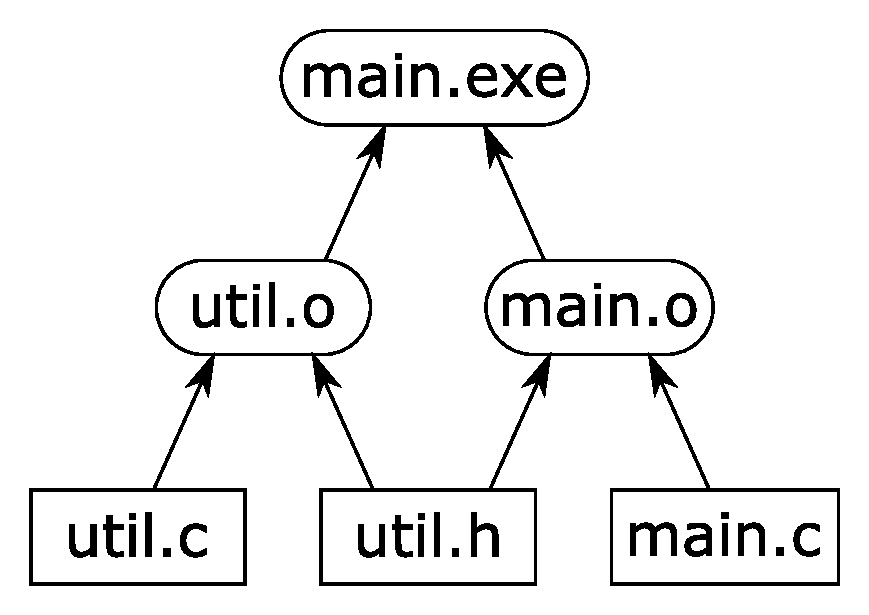
\includegraphics[scale=0.28]{fig/make-example.pdf}}
\caption{Task dependency graph}
\end{subfigure}
\begin{subfigure}[b]{0.32\linewidth}
\centerline{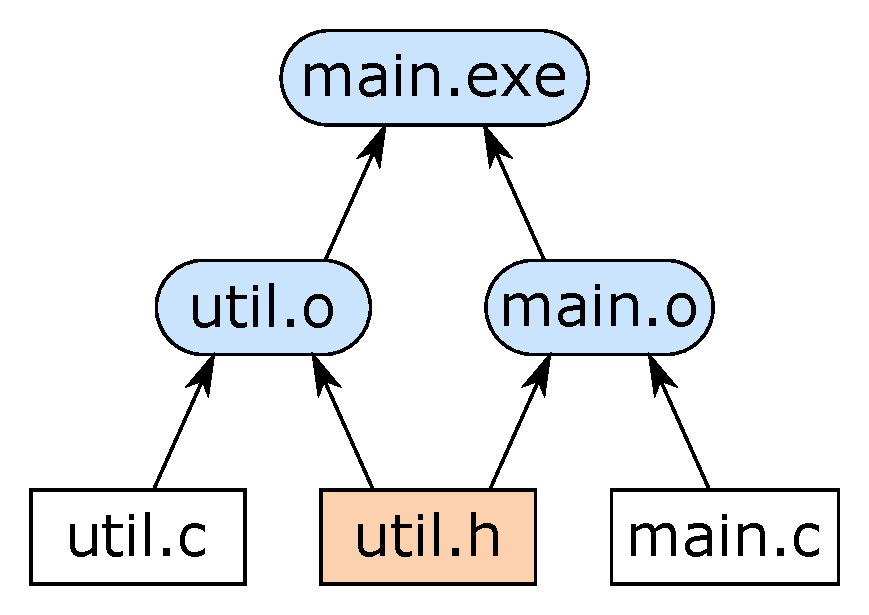
\includegraphics[scale=0.28]{fig/make-example-full.pdf}}
\caption{Full rebuild}
\end{subfigure}
\begin{subfigure}[b]{0.32\linewidth}
\centerline{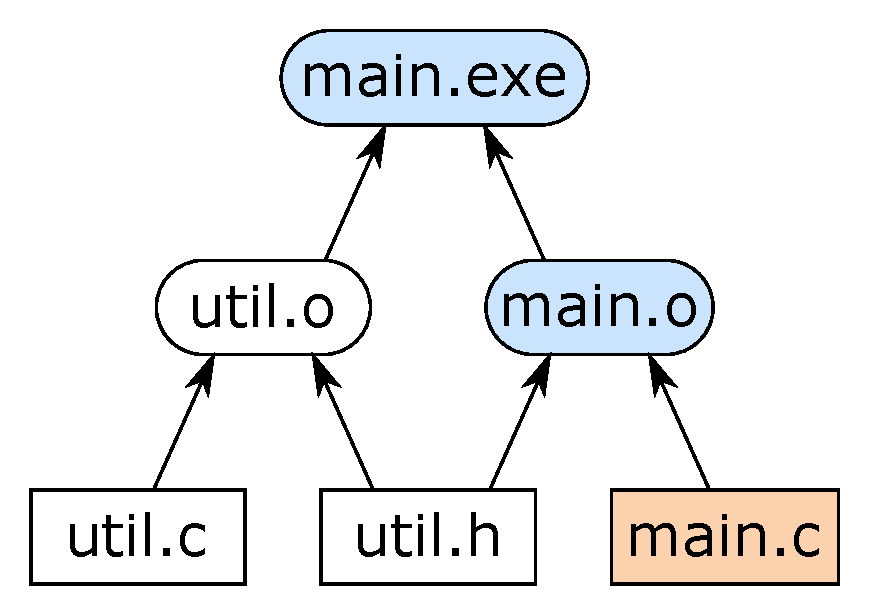
\includegraphics[scale=0.28]{fig/make-example-partial.pdf}}
\caption{Partial rebuild}
\end{subfigure}
\caption{A task dependency graph and two build scenarios. Input files are shown as
rectangles, intermediate and output files are shown as rounded rectangles. Dirty
inputs and files that are rebuilt are highlighted.
\label{fig-make}}
\end{figure}

If the user modifies the sources of the utility library and runs \Make, it will
perform a full rebuild, because all three tasks transitively depend on the
library, as illustrated in Fig.~\ref{fig-make}(b). On the other hand, if the
user modifies \cmd{main.c} then a partial rebuild is sufficient: indeed, the
file \cmd{util.o} does not need to be rebuilt, since its inputs have not
changed, see Fig.~\ref{fig-make}(c). Files that have changed since the previous
build are called \emph{dirty}.

The requirement to \emph{execute tasks at most once and only if they transitively
depend on dirty inputs} is essential for build systems, it is their raison
d'\^etre. We will call build systems that satisfy this requirement \emph{minimal}.

To achieve minimality \Make relies on two main ideas. First, it uses \emph{file
modification time} to detect the files that are dirty: a file is marked dirty if
it was modified since the previous build. Second, it constructs a complete task
dependency graph from the information contained in the makefile and executes
tasks in a \emph{topological order}.

Note that it is not always possible to know the dependencies of a task upfront,
or \emph{statically}. To demonstrate this, let us add another task to the above
makefile:

\vspace{1mm}
\begin{minted}[xleftmargin=10pt]{makefile}
release.tar: main.exe README
    tar -cf release.tar main.exe README
\end{minted}
\vspace{1mm}

\noindent
So far so good: if either \cmd{main.exe} or \cmd{README} is dirty, \Make will
recreate the release archive. But now imagine that we need to specify the files
that go into \cmd{release.tar} in a text file \cmd{release.txt}. The dependencies
of \cmd{release.tar} are no longer known statically: they \emph{depend on the
contents} of \cmd{release.txt}, which might not even exist before the build
starts, e.g. if it is produced by concatenating input files \cmd{release-bins.txt}
and \cmd{release-docs.txt}. Alas, makefiles cannot express such \emph{dynamic
dependencies}, requiring ad hoc workarounds such as \emph{build phases}, which
are problematic~\cite{hadrian}.

\subsection{\Excel: dynamic dependencies at the cost of minimality}
\label{sec-background-excel}

\Excel is a build system that can deal with dynamic dependencies albeit at the
cost of sacrificing minimality. Consider the following spreadsheet comprising
four input cells \cmd{A1-A3} and \cmd{B1}, and a single task computing the sum
of values \cmd{A1} $+\cdots+$ \cmd{An}, where \cmd{n} is specified indirectly in
\cmd{B1}:

\vspace{1mm}
\begin{minted}[xleftmargin=10pt]{bash}
A1 = 10
A2 = 20
A3 = 30
B1 = 2
C1 = SUM(A1:INDIRECT("A" & B1))
\end{minted}
\vspace{1mm}

\noindent
The output \cmd{C1} here is analogous to the \cmd{release.tar} from the previous
example: one cannot statically determine the dependencies of the associated task.
To deal with this, \Excel takes a simple conservative approach: it marks all
cells with dynamic dependencies as dirty and therefore always recomputes them
during a rebuild. This guarantees that the build result is correct, but clearly
violates the minimality requirement: if the user modifies \cmd{A3}, \Excel will
recompute \cmd{C1} even though it does not transitively depend on \cmd{A3}.

Note that \Excel's approach to marking cells as dirty is a relatively minor
variation of the approach used by \Make: a cell is considered dirty if it was
modified since the previous build \emph{or if it is volatile}, where the notion
of volatility includes dynamic dependencies, as well as \emph{non-determinism}
that will be discussed in~\S\ref{sec-engineering}. We therefore put both \Make
and \Excel in the same category of build systems that associate a \emph{dirty bit}
with every file or cell. (To avoid the ``file or cell'' nuisance, we introduce the
abstract notion of \emph{keys} in~\S\ref{sec-background-vocabulary}.)

\Excel's recalculation algorithm~\cite{excel_recalc} on the other hand is
significantly different from \Make. Since it is impossible to construct the full
dependency graph upfront in the presence of dynamic dependencies, \Excel
maintains the \emph{calculation chain}, which is an approximation to the correct
topological order. During recalculation, \Excel processes cells in this order,
but can \emph{defer recalculation of a cell} by moving it down the chain when newly
discovered dynamic dependencies dictate that. We discuss this algorithm in more
detail in~\S\ref{sec-examples}.

Another distinguishing feature of \Excel is \emph{self-tracking}. Most build
systems track changes of inputs and intermediate results, executing dependent
tasks whenever they change, but \Excel can also track changes in the tasks
themselves: if a formula is modified, \Excel will recompute it and propagate
the changes. Self-tracking is uncommon in software build systems, where one
often needs to manually initiate a full rebuild even if just a single task has
changed.

\subsection{\Shake: dynamic dependencies with no remorse}
\label{sec-background-shake}

\Shake was developed specifically to address the issue of dynamic
dependencies~\cite{mitchell2012shake} and it excels at handling them without
sacrificing the minimality requirement. Here is how one can express the task
for producing \cmd{release.tar} from the example discussed
in~\S\ref{sec-background-make}.

\vspace{1mm}
\begin{minted}[xleftmargin=10pt]{haskell}
"release.tar" %> \_ -> do
    need ["release.txt"]
    contents <- lines <$> readFile "release.txt"
    need contents
    system "tar" $ ["-cf", "result.tar"] ++ contents
\end{minted}
\vspace{1mm}

\noindent
We first declare the static dependency on \cmd{release.txt}, then read its
content and depend on it, dynamically. Finally, we specify the command to
produce the resulting archive. Crucially, the archive will only be rebuilt if
one of the dependencies (static or dynamic) has changed.

\todo{AM}{How is \Shake different.}

\begin{figure}[h]
\centerline{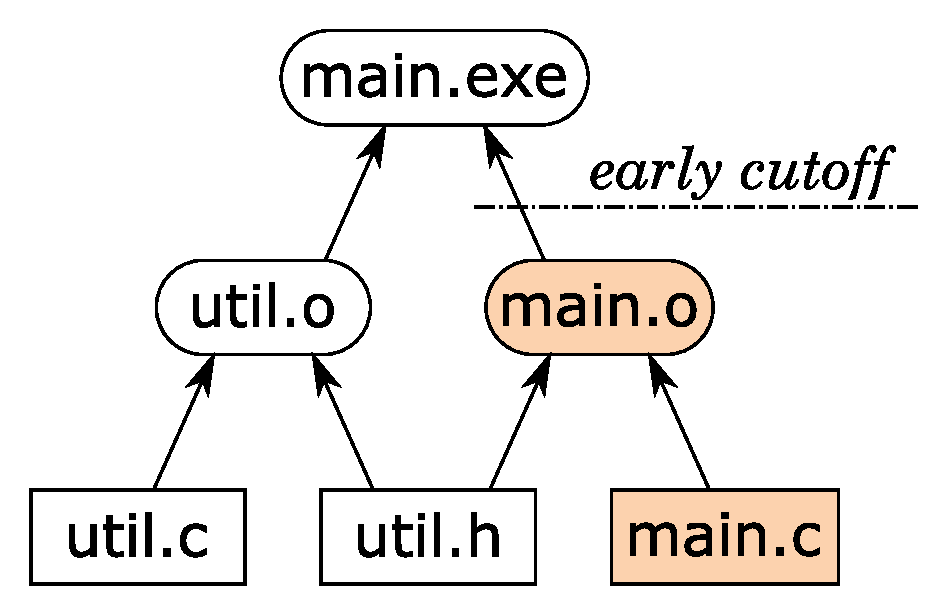
\includegraphics[scale=0.28]{fig/make-example-cutoff.pdf}}
\vspace{-2mm}
\caption{An early cutoff example: modify the source \cmd{main.c} by adding a
comment. The rebuild is stopped after detecting that \cmd{main.o} is unchanged,
which indicates that \cmd{main.exe} does not need to be rebuilt.\label{fig-cutoff}}
\end{figure}

\Shake also supports the following \emph{early cutoff optimisation}. When it
executes a task and the result is unchanged from the previous build, it is
unnecessary to execute the dependent tasks, and hence \Shake can stop a build
earlier, as illustrated in Fig.~\ref{fig-cutoff}. Not all build systems support
early cutoff: \Make and \Excel do not, whereas \Shake and \Bazel (introduced
below) do.

...

\subsection{\Bazel: a cloud build system}
\label{sec-background-shake}

When build systems are used by large teams, different team members
often end up executing exactly the same tasks on their local machines.
A \emph{cloud build system} can speed up builds dramatically by
transparently sharing build results among team members. Furthermore, cloud
build systems allow one to perform \emph{shallow builds} that materialise
only end build products on a local machine, leaving all intermediates in the
cloud. This is a significant optimisation compared to \emph{deep builds}
that require all transitive dependencies of an end build product to be
locally available. Non-cloud build systems cannot support shallow builds.

\subsection{Abstract vocabulary for build systems}
\label{sec-background-vocabulary}

\subsection{Keys, values, hashes and store}

Keys are
used to distinguish values. In build systems keys are typically filenames, e.g.
\cmd{main.c}, whereas values are file contents (a C program source code in this
case). In spreadsheets keys are cell names, e.g. \cmd{A1}, and values are
numbers, text, etc. that are typically displayed inside cells. In Haskell code,
we will use type variables \hs{k} and \hs{v} to denote keys and values,
respectively.


A \emph{store} associates keys to values. It is convenient to assume that a store
is total, i.e. it contains a value for every possible key. We therefore also
assume that the type of values is capable of encoding values corresponding to
non-existent keys (missing files or empty cells).

We use a cryptographic \emph{hash function} \hs{hash :: v -> Hash} for
efficient tracking and sharing of build results.

\subsection{Input, intermediate and output values}

Some values must be provided by the user as \emph{input}. For example,
\textsf{src/file.c} can be edited by the user who relies on the build system to
compile it into \textsf{obj/file.o}. Similarly, the user can input \textsf{A1 = 5}
and \textsf{B1 = 9} expecting the spreadsheet to compute their sum in \textsf{C1},
i.e. \textsf{C1 = 14}.

In the above examples, \textsf{obj/file.o} and \textsf{C1} are \emph{output} values.

In some situations we might also need the notion of \emph{intermediate} values,
which are not interesting for the user but are produced in the process of turning
inputs into outputs. For example, the user might only be interested in the
executable \textsf{bin/file.exe} obtained by linking \textsf{obj/file.o} with
standard libraries, in which case \textsf{obj/file.o} can be considered an
intermediate value.

\subsection{Non-deterministic computations}

Build systems and spreadsheets compute output values from input and intermediate
values. In the most typical case, these \emph{computations} are \emph{functions},
such as \textsf{C1 = A1 + B1}, i.e. their result is uniquely determined by the
input values. However, in general they can be \emph{relations}, i.e. have
multiple valid results. A spreadsheet example: \textsf{A2 = A1 + RANDOM(1,6)}.
This computation has six valid results for each input value \textsf{A1}. In
build systems, the object file \textsf{obj/file.o} is sometimes not uniquely
determined by the source \textsf{src/file.c} -- different compiler runs may
produce different valid results.


\begin{itemize}

    \item Some build systems, e.g. \Buck, require all tasks to be
    \emph{deterministic}, i.e. produce exactly the same output when run on the
    same inputs. However, not all tasks are deterministic, and there are build
    systems that support \emph{non-determinism}. A simple example is \Excel's
    \textsf{RANDBETWEEN(low, high)} that returns a random integer in the
    interval \textsf{[low, high]}.

    \item Most build systems persistently store auxiliary \emph{build
    information} for profiling and optimisation purposes: \Make stores file
    modification times, \Shake stores the discovered dynamic dependency graph,
    \Bazel and other cloud build systems store information about inputs and
    outputs of previously executed tasks, etc.
\end{itemize}

This paper presents a purely functional abstraction for build systems that
allows us to express all the above intricacies of build systems and design
complex build systems from simple primitives. The presented abstraction fits in
just two lines of Haskell code, which are explained
in~\S\ref{sec-abstractions}:

\begin{minted}{haskell}
type Compute c k v = @\std{forall}@ f. c f => (k -> f v) -> k -> Maybe (f v)
type Build c i k v = Compute c k v -> k -> Maybe i -> Map k v -> (i, Map k v)
\end{minted}


Below we define basic notions used in build systems and other similar domains,
for example, spreadsheets.


\subsection{Requirements for build systems}

\begin{itemize}
    \item Correctness
    \item Minimality
    \item Support for sharing and skipping intermediate values
\end{itemize}
...

\clearpage

\section{Build systems, abstractly}\label{sec-build-abstractions}

In this section we present the \emph{compute} and \emph{build} abstractions:
\begin{itemize}
    \item Compute represents build rules (in build systems) or formulas (in
    spreadsheets), and is completely isolated from the world of compilers, file
    systems, memories, caches, and all other complexities of real build systems.
    \item Build corresponds to the algorithm used for bringing a key-value store
    to a coherent state by running compute.
\end{itemize}

\begin{figure}
\begin{minted}{haskell}
type Compute f k v = (k -> f v) -> k -> f (Maybe v)

type FunctorialCompute  f k v = Functor     f => Compute f k v
type ApplicativeCompute f k v = Applicative f => Compute f k v
type AlternativeCompute f k v = Alternative f => Compute f k v
type MonadicCompute     f k v = Monad       f => Compute f k v
type MonadPlusedCompute f k v = MonadPlus   f => Compute f k v
\end{minted}
\caption{Compute abstractions}\label{fig-compute}
\end{figure}

Consider abstractions in Fig.~\ref{fig-compute}.

...

We now describe several types of build systems according to their constraint
on the functor \hs{f}.

...


\clearpage
\section{Build systems, concretely}\label{sec-examples}

This section present several concrete examples of build systems, providing
simple implementations that use the previously introduced abstractions.

\subsection{Applicative build systems}

Applicative build system can only accept an applicative compute, because they
rely on building the full dependency graph upfront, which is impossible with
dynamic dependencies.

\vspace{4mm}
\subsubsection{An incorrect applicative build system}~\\

\todo{AM}{Describe the \hs{dumbBuild} that builds outputs in the given order.}

\vspace{4mm}
\subsubsection{\Make: a correct but non-minimal applicative build system}~\\

We start by applicative build systems, such as the classic vanilla
\Make\footnote{There are numerous implementations of \Make and none comes with a
formal specification. In this paper we therefore use a simple but reasonable
approximation to a real \Make that you might find on your machine.} and a more
recent \Ninja.

Make is correct but non-minimal. It is unusual from other build systems in that
it relies on \emph{timed values}, i.e. on a map \hs{age :: v -> Time}, as a
heuristic to decide whether a value is up-to-date.

\todo{NM}{Add a description of \Make.}

\vspace{4mm}
\subsubsection{\Ninja: a correct and minimal applicative build system}~\\

\Ninja is a modern alternative to \Make ...

\todo{NM}{Add a description of \Ninja.}

\todo{AM}{What about Nix? John Ericson suggested in a blog comment that it may
be somewhat monadic, see:
\url{https://blogs.ncl.ac.uk/andreymokhov/cloud-and-dynamic-builds/\#comment-1849}.}

\subsection{Monadic build systems}

...
\subsubsection{An incorrect monadic build system}~\\

See \hs{dumbBuild}.

\subsubsection{Correct but not minimal monadic build system}~\\

As of writing, XXX is a correct but non-minimal monadic build system. Here is
an example where it does unnecessary computation:

\begin{minted}[frame=single]{text}
A1 = 10
A2 = MIN(A1, 4)
A3 = SQRT(A2)
\end{minted}

After performing the build, XXX computes \textsf{A2 = 4} and \textsf{A3 = 2}
from the input cell \textsf{A1}. Now if the user changes the \textsf{A1} to 5,
XXX will recompute both \textsf{A2 = 4}, which is necessary, but also
\textsf{A3 = 2}, which is unnecessary since its only dependency (\textsf{A1})
has not changed since the previous build.

One possible implementation of a spreadsheet build
system\footnote{For example, see \url{http://www.decisionmodels.com/calcsecretsc.htm}.}
is to maintain a
sequence of cells in which they should be evaluated. The build system takes this
sequence as input, marks all cells as \emph{unevaluated}, and then attempts to
evaluate all cells in the order specified by the sequence. If the cell to be
evaluated depends on an unevaluated cell, this means the provided sequence is
not a correct topological order and is updated by moving the current cell to the
back of the sequence. The build then proceeds with the next cell. Otherwise, if
all dependencies of the current cell have been marked as \emph{evaluated}, the
build system computes the correct value for the cell by evaluating the formula,
writes it into the spreadsheet and proceeds to the next cell in the sequence. If
there are no cyclic dependencies, this process eventually terminates with
correct results. The resulting sequence, which is guaranteed to respect the
topological order of dependencies is stored to be reused during the next build.

...

Interesting note: XXX is unusual in that it tracks changes in the compute,
i.e. if a user edits a formula, XXX will correctly rebuild results. Most build
systems, including \Shake, do not meet this requirement and a clean rebuild may
be necessary if the user edits build rules.

...

\subsubsection{Correct and minimal monadic build system}~\\

\Shake is a correct and minimal monadic build system.
\todo{NM}{Describe \Shake using our abstractions.}

\subsection{Cloud build systems}

Codebase of large software projects comprises millions of lines of code spread
across thousands of files, each built independently by thousands of developers
on thousands of machines. A distributed cloud build system speeds up builds
dramatically (and saves energy) by transparently sharing build products among
developers.

\todo{AM}{Also mention YYY (developed by ZZZ), Buck (Facebook) and Pants
(Twitter et al). Buck is essentially the same. Are they essentially the same?}

\Bazel is a cloud build system developed by Google, which supports caching of
build results. To achieve that, it maintains two partial maps:

\begin{minted}{haskell}
type Cache =  Hash  -> Maybe v
type Known = [Hash] -> Maybe Hash
\end{minted}

\hs{Cache} is a conventional \emph{content-addressable store}, that can be used
to fetch a previously computed value given its hash.

\hs{Known} records a known outcome of a computation that took a list of values
as input (represented by their hashes) and produced a resulting value (also
represented by its hash). Now, a build system has the following two options to
recompute a value:

\begin{itemize}
    \item Call the compute function on the store containing all up-to-date
    dependencies and put the computed value to the store.
    \item Collect hashes of all up-to-date dependencies \hs{hs} and query the
    \hs{Known} map. If this computation has been performed before, the map will
    contain the hash \hs{h} of one valid result (recall that the compute function
    may be non-deterministic). It is now possible to lookup \hs{h} in the
    \hs{Cache} and if it contains a value \hs{v} it can be downloaded to the
    local store instead of running the compute.
\end{itemize}

...

\todo{AM}{Also describe the XYZ algorithm.}


%% Acknowledgments
\begin{acks}
  %% acks environment is optional
  %% contents suppressed with 'anonymous'
  %% Commands \grantsponsor{<sponsorID>}{<name>}{<url>} and
  %% \grantnum[<url>]{<sponsorID>}{<number>} should be used to
  %% acknowledge financial support and will be used by metadata
  %% extraction tools.
  We would like to thank ...
\end{acks}

% \bibliography{refs}

%% Appendix
% \appendix
% \section{Appendix}
% Text of appendix \ldots

\end{document}
